\documentclass[notes]{beamer}
\usepackage{graphicx}
\usetheme{Warsaw}
\title{Cluster Scheduling}
\author{Inigo Mediavilla}
\date\today
\setbeamertemplate{note page}[plain]

\graphicspath{ {./images/} }

\begin{document}

  \begin{frame}
  \titlepage
  \end{frame}
  
  \note{}

  \begin{frame}
    \frametitle{Scheduling}
    \begin{definition}{Scheduling:}
    planning the execution of a set of computations that
    are called jobs in an execution environment with a limited amount
    of resources.
    \end{definition}
    \begin{itemize}
      \item Why is it relevant?
      \begin{itemize}
        \item Growing datacenters for big companies (Google, Yahoo!,
          Facebook, Amazon)
        \item Small and Medium sized companies own more clusters (in
          the cloud or physically)  
        \item Increasing popularity of distributed processing
      \end{itemize}
    \end{itemize}
  \end{frame}

  \note{}

  \begin{frame}
    \frametitle{Why is it difficult?}
    \begin{itemize}
      \item Increasing size of clusters
      \item Growing number of jobs to run
      \item Jobs are more sensitive to scheduling delays
      \item Diversity of scheduling needs
    \end{itemize}
  \end{frame}

  \note{}

  \begin{frame}
    \frametitle{Different Approaches}
    \begin{itemize}
      \item Centralized Scheduler (single-path or multi-path)
      \item Static partitioning
      \item Two level Schedulers (i.e. Mesos)
      \item Optimistic locking (i.e. Omega)
    \end{itemize}
  \end{frame}

  \note{}

  \begin{frame}
    \frametitle{Centralized Scheduler}
    \begin{columns}[T]
       \begin{column}{.5\textwidth}
        \begin{block}{Advantages/Disadvantages}
            \begin{itemize}
              \item[+] Initially simple
              \item[+] Efficient policies with few frameworks
              \item[-] Scalability problems: scheduler is a bottleneck
              \item[-] Head of line blocking (even with multi-path)
              \item[-] Can't deal with different scheduling needs
            \end{itemize}
   % Your text here
        \end{block}
       \end{column}
       \begin{column}{.6\textwidth}
   % Your image included here
         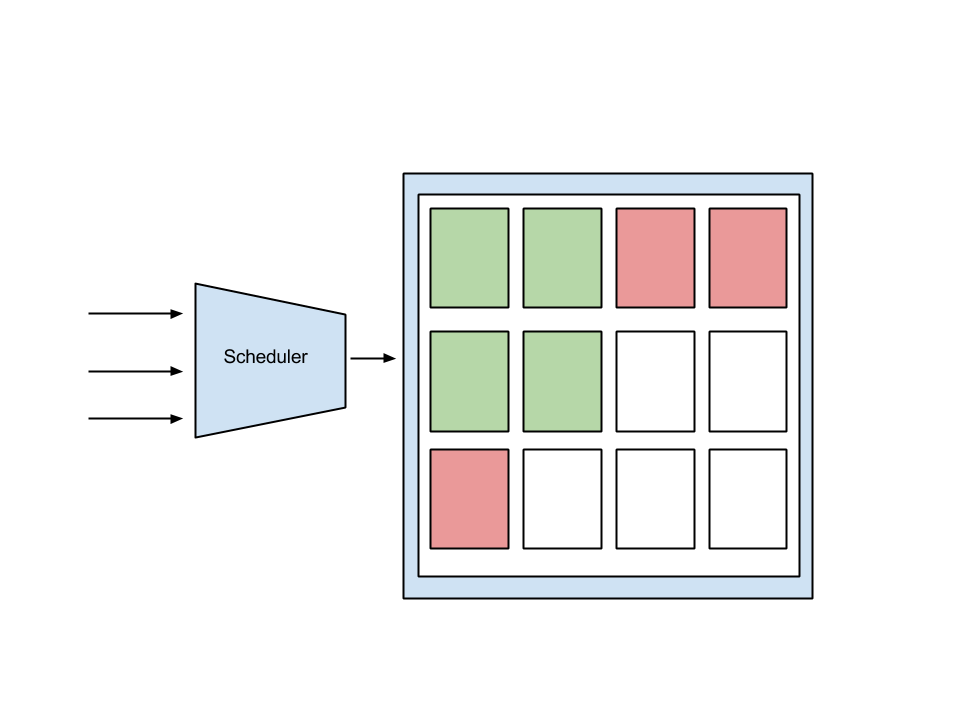
\includegraphics[trim = 0mm 0mm 50mm 0mm,clip,scale=0.20,natwidth=960,natheight=720]{CentralizedScheduler.png}
       \end{column}
     \end{columns}
  \end{frame}

  \note{}

  \begin{frame}
    \frametitle{Static partitioning}
       \begin{columns}[T]
       \begin{column}{.5\textwidth}
        \begin{block}{Advantages/Disadvantages}

            \begin{itemize}
              \item[+] Frameworks can schedule the way they want 
              \item[+] No possibility of conflicts
              \item[-] Really inefficient use of the cluster
            \end{itemize}
        \end{block}
        \end{column}
        \begin{column}{.6\textwidth}
         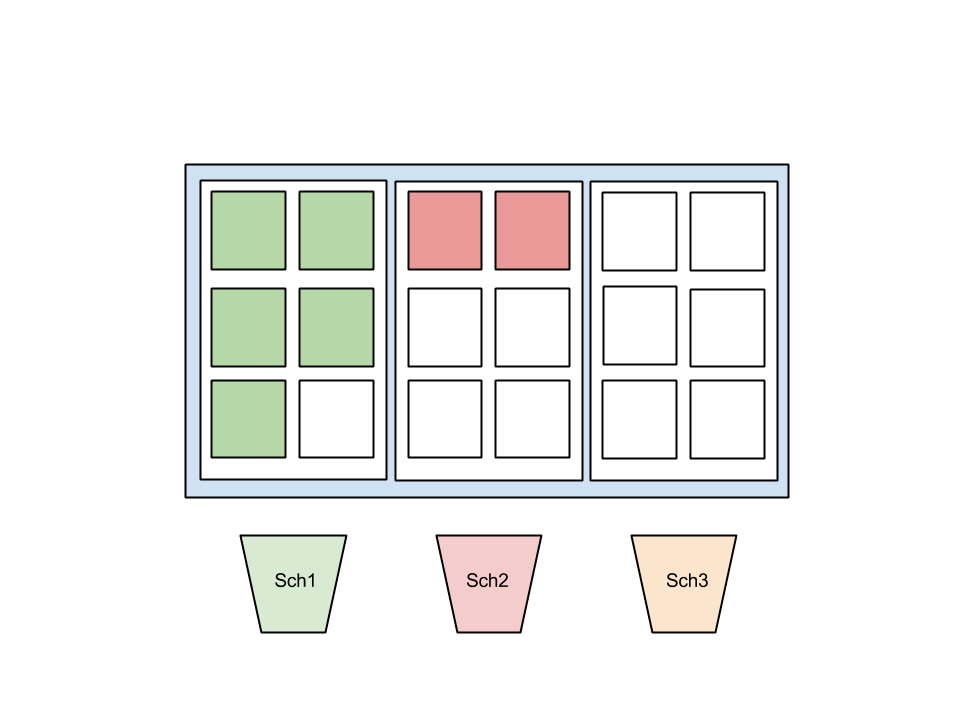
\includegraphics[trim = 0mm 0mm 50mm 0mm,clip,scale=0.20,natwidth=960,natheight=720]{StaticPartitioning.png}
        \end{column}
      \end{columns}
  \end{frame}

  \note{}

  \begin{frame}
    \frametitle{Two-Level Scheduler}
    \begin{definition}
      A central scheduler offers the available resources to
      the frameworks that can accept them and launch tasks
      with them.
    \end{definition}
    \begin{itemize}
      \item Resources are dynamically allocated
      \item Frameworks schedule tasks the way they want
        with the resources they get
    \end{itemize}
  \end{frame}

  \note{}

  \begin{frame}
    \frametitle{Two-Level Scheduler - Pros and Cons}
       \begin{columns}[T]
       \begin{column}{.5\textwidth}
        \begin{block}{Process}
           Frameworks receive offers for the available resources 
           from the scheduler. 
        \end{block}
        \begin{block}{Advantages/Disadvantages}
            \begin{itemize}
              \item[+] Resources are no longer compartimented
              \item[+] No possibility of conflicts
              \item[-] Long frameworks slow down the cluster
              \item[-] Two frameworks hoarding resources can provoke a deadlock
            \end{itemize}
        \end{block}
        \end{column}
        \begin{column}{.6\textwidth}
         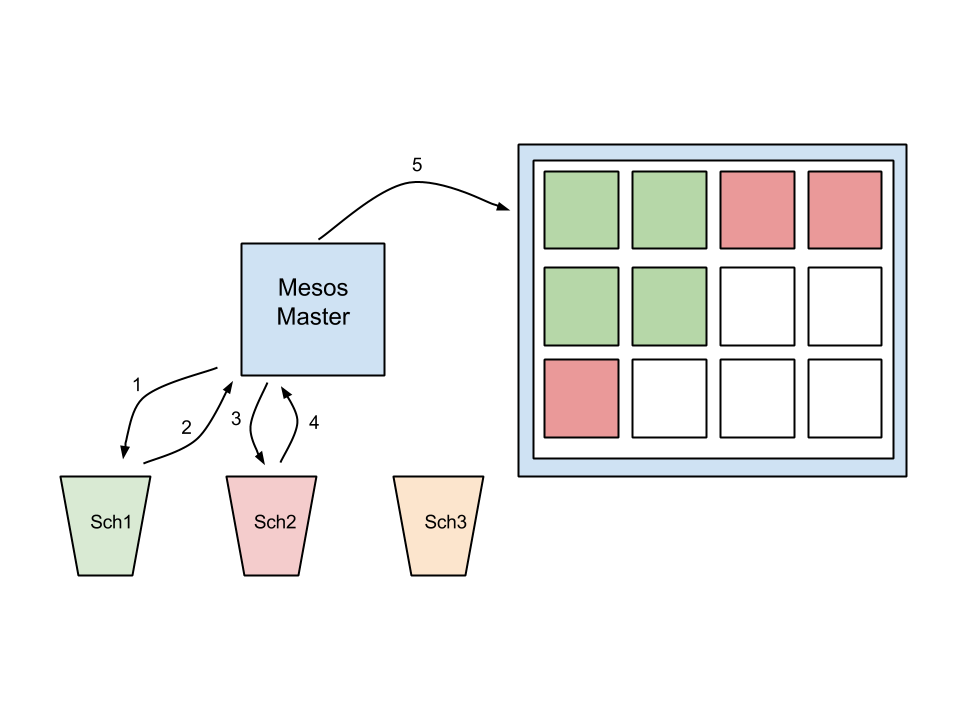
\includegraphics[trim = 0mm 0mm 10mm 0mm,clip,scale=0.18,natwidth=960,natheight=720]{TwoLevel.png}
        \end{column}
      \end{columns}
  \end{frame}

  \note{}

  \begin{frame}
    \frametitle{Omega Scheduler}
    \begin{definition}
      Every framework knows the state of the cluster that
      is updated only by the scheduler. The scheduler's role
      is just to mediate when conflict happens and share
      the state of the cluster with the frameworks when updates
      happen.
    \end{definition}
  \end{frame}

  \note{}


  \begin{frame}
    \frametitle{Omega Scheduler - Advantages}
    \begin{itemize}
      \item[+] Frameworks don't hold locks
      \item[+] Inactive frameworks don't interfere
      \item[+] Slow scheduling frameworks don't block others
      \item[+] Frameworks can dynamically adjust their effort when 
            the cluster is not busy
      \item[-] No implementation proposed
      \item[-] No fairness mechanism (proposed priorities and post-facto monitoring)
    \end{itemize}
  \end{frame}

  \note{}

  \begin{frame}
    \frametitle{Contributions}
    \begin{itemize}
        \item Prototype implementations of Mesos and Omega
        \item Study of Offer-all vs Fair share alternatives for Mesos
        \item Simulation optimistic locking with Mesos (and the other way around)
        \item Fairness and Data-locality proposition for Omega
    \end{itemize}
  \end{frame}

  \note{}

  \begin{frame}
    \frametitle{Prototype implementations}
    \begin{itemize}
        \item Omega's is first proposed implementation
        \item Allow to:
        \begin{itemize}
          \item Study the two different models
          \item Spot similarities - Propose common models (e.g
            cross-model simulations)
          \item Test features
          \item Test performance
          \item Test general solutions in the two models 
        \end{itemize}
        \item Simplifications
          \begin{itemize}
            \item Frameworks are really simple internal processes (no
              different scheduling needs emulated)
            \item Tasks aren't run distributedly (just in their own thread)
            \item No high volumes of traces run against the prototypes
          \end{itemize}
    \end{itemize}
  \end{frame}

  \note{}

  \begin{frame}
    \frametitle{Study of Offer-all vs Fair share alternatives}
    \begin{itemize}
      \item Nothing
    \end{itemize}
  \end{frame}

  \note{}

  \begin{frame}
    \frametitle{Simulating optimistic locking with Mesos}
    \begin{itemize}
      \item How does it work?
      \item Requirements
      \item Advantages, Disadvantages
      \item Interest of Mixed strategy
    \end{itemize}
  \end{frame}

  \note{}

  \begin{frame}
    \frametitle{Fairness and datalocality proposition for Omega}
    \begin{itemize}
      \item Fairness (quick explanation of DRF)
      \item Limitations of DRF (and other fairness algorithms)
      \item How to get both fairness and locality? Delay Scheduling
      \item Delay scheduling implementation for Omega
    \end{itemize}
  \end{frame}

  \note{}

\end{document}
%Final Goals


%  - Mainly two types of jobs with completely different requirements:


%    (why is it difficult for a scheduler to schedule service jobs and batch jobs?
%     because the kind of needs that a service can have are usually different to 
%     those of batches (who usually need mainly datalocality and low latency for
%     task assignment), so the dificulty is more that a scheduler has to respond
%     to completely heterogenous needs)
     
%    - Service jobs: long running, resource consuming, require low-latency, high availability
%    - Batch jobs: 
%      - short running, to finish as soon as possible 
%      - splitted in multiple smaller tasks that can be usually parallelized and distributed 
%      (They usually process data that is distributed across a cluster so they benefit from data locality (explain what it is), 
%      - represent around 80% of the jobs in a cluster 
%      - cannot afford delays in the scheduling

%  - Maximize the utilization of the cluster

%Challenges:

%  - Heterogenous applications with different scheduling needs (e.g Hadoop vs MPI)
%  - Duplicating the cluster's data is expensive and may bring synchronization problems
%  - Scalibility and high availability (the scheduler needs to be able to be able to keep serving quickly enough as the cluster grows and it cannot afford long downtimes)

%One or many schedulers?

%Requirements for a scheduler

%  - Respond to scheduling needs (job constraints)
%  - Be flexible to respond to the different needs of the frameworks that will run in the cluster
%  - Be quick (delays will affect the performance of the cluster. e.g delays in scheduling
%    hadoop tasks can really affect the performance since there are thousands of task per job)
%  - Scale when the cluster grows
%  - Be simple (Ideally)



%  \begin{frame}
%    \frametitle{Goals}
%    \begin{itemize} 
%     \item Execute Jobs within given constraints
%       \begin{itemize}
%         \item Two different kinds of jobs (services and batch jobs)
%         \item Types of job constraints
%         \begin{itemize}
%           \item Execution time
%           \item High availability
%           \item Failover
%           \item Data locality
%         \end{itemize}
%       \end{itemize}
%     \item (Secondary) Maximize cluster utilization
%    \end{itemize}
%    %Content goes here
%  \end{frame}
%  \begin{frame}
%    \frametitle{Difficulties}
%    \begin{itemize}
%      \item Scheduler needs to scale as the cluster grows
%      \item Scheduler needs to be highly available
%      \item Heterogenous mixed of jobs to execute 
%            (batch/services, hadoop vs MPI, ..)
%            \em (Different scheduling needs) 
%      \item New data processing frameworks demand subsecond scheduling times for 
%            their tasks
%      \item Ideally the scheduler needs to be simple
%    \end{itemize}
%    %More content goes here
%  \end{frame}
%  \begin{frame}
%    Existing scheduling solutions
%    \begin{itemize}
%      \item Centralized Scheduler
%%      \item Static Partitioning
%      \item Two-level phase scheduler (Mesos, YARN)
%      \item Distributed optimisted locking scheduler (Omega)
%      \item Fully distributed scheduler (Sparrow) - Specialized for data processing
%            jobs
%%    \end{itemize}
%  \end{frame}
%  \begin{frame}
%    \begin{itemize}
%%      \item Centralized Scheduler
%      \begin{itemize}
%        \item Pros
%%        \begin{itemize}
%          \item Control over the whole cluster
%%          \item Can achieve good cluster utilization
%          \item Can be simple when there's only one framework running in the cluster
%        \end{itemize}
%%%      \end{itemize}
%      \begin{itemize}
%        \item Cons
%%        \begin{itemize}
%          \item Single point of failure
%          \item Doesn't scale (bottleneck)
%          \item It becomes really complex with an environment where many kinds of 
%                jobs are executed
%          \item It doesn't scale well
%        \end{itemize}
%      \end{itemize}
%    \end{itemize}
%
%  \end{frame}



